\subsection{Creative Mode}
For the creative mode task we chose to place a face mask on every face found in an image. This was implemented in function \textbf{fnPandemicMode}. 
 
We used the \textbf{roipoly} method to define a polygonal region of interest in the original face mask image (facemask-cropped.jpg). we then scaled the face mask image and the polygonal region of interest with respect to cropped face image size. We then created "positive" and "negative" segmentation mask matrices, to add or remove the face mask image or region as required. The dot product between the cropped face image and the negative mask matrix removed the face mask region, all black colour values in that region being equal to zero. This resulting matrix was then added to the positive mask, containing the face mask image surrounded by a blacked out region.  

To define where the mask would be placed, our initial approach was to use a mouth locating feature from MATLAB object \textbf{vision.CascadeObjectDetector}. We did not find this approach robust, as returned mouth locations varied between nose and chin. In the end we found it simpler to display the mask at a fixed ratio from the bottom edge and mid-point between side edges of cropped face.

On the top row of Figure \ref{fig:pandemic_mode}, the middle image represents the negative segmentation mask. A dot product with the cropped face on left-hand size image creates a black void in the face mask area on right-hand side image. On the bottom row, the middle image represents the positive segmentation mask, which is added to "voided" left-hand side image, resulting in void being filled by face mask on right-hand side image. These were the concepts used for prototyping, in practice we removed a section from cropped face, performed the matrix operations and inserted the resulting section back into the original image.

\begin{figure}[h]
 \centering 
 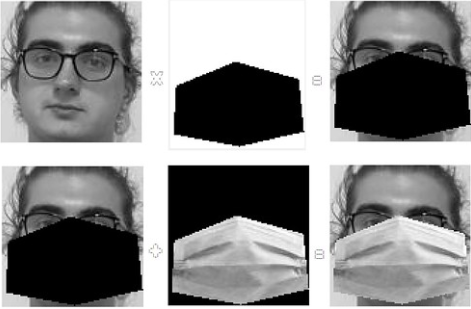
\includegraphics[width=\columnwidth]{images/PandemicMode.png}
 \caption{Creative Mode superimposing facemask on face image}
 \label{fig:pandemic_mode}
\end{figure}